\documentclass{edm_template}
\usepackage{subfig}

\begin{document}

\title{Mining Frequent Learning Pathways from a Large Educational Dataset}

\numberofauthors{3}
%
\author{
Nirmal Patel \\ \affaddr{Playpower Labs} \\ \email{nirmal@playpowerlabs.com} \and
Collin Sellman \\ \affaddr{Arizona State University} \\ \email{collin.sellman@asu.edu} \and
Derek Lomas \\ \affaddr{Playpower Labs} \\ \email{derek@playpowerlabs.com}
}

\maketitle
\begin{abstract}
In this paper, we describe data mining techniques used to extract frequent learning pathways from a large educational dataset. These pathways were extracted as a directed graph. By filtering the graph, we found that amid various learning pathways that students took, there were certain pathways that were more frequent than others. These pathways represented \textit{highways} of student learning. Our original dataset contains more than 800 million interactions of over 3 million anonymized students. For the analysis presented in this paper, we randomly sampled 20,000 students from a grade 3 math program. Prior to extracting the learning pathway graph, we used a sequence clustering technique to group together students with similar learning pathways. This allowed us to reduce the complexity of the graph.
\end{abstract}

\section{Introduction}
Digital learning platforms collect a wide variety of student interaction data. These data can be used to inform continuous improvement at the level of the product, school district, classroom or the individual student. Recently, we've begun to investigate individual sequences of instructional content, which we call "learning pathways" or "student journeys."  Using  various data mining techniques, we've analyzed the learning pathways from thousands of students, revealing the emergence of interesting patterns and structures.

By using newly developed process mining techniques, we can look for process models of student learning \cite{mukala2015exploring, trcka2010process}. Such models can be used to discover usage patterns or to compare usage to ideal patterns. Unfortunately, when working with data from many thousands of students, we find that there are too many underlying processes. Therefore, the resulting process models show "spaghetti": an unintelligible mess of various processes. Process discovery algorithms like Fuzzy Mining can help reduce the spaghetti \cite{gunther2007fuzzy}, but they render models that are not amenable to extensive manipulation or enhancement.

To address these issues, we first explored sequence clustering techniques to see if they could help us identify groups of students who follow similar processes \cite{hompesdiscovering}. We developed an edit distance based clustering algorithm, which allowed us to group together students with similar learning pathways. Using this technique on our sample of 20,000 students, we discovered three distinct groups of students that differed in their length of learning paths. Then, we implemented and applied a graph-based process discovery algorithm on these clusters to extract directed graphs that revealed to us frequent learning pathways that students took. We found that our graph-based process models were easy to manipulate and enhance.

The rest of the paper is structured as follows. In section 2, we describe the dataset which we used for data mining. In section 3, we briefly describe the sequence clustering algorithm we used on data and discuss the results. In section 4, we succinctly describe the graph mining algorithm we used to discover a directed graph encoding student learning pathways. We filtered this graph to find frequent paths. At the end, we discuss the usefulness of techniques presented in this paper, and directions for future work.

\section{Dataset}
Our original dataset is formatted as an event log. Each row of the dataset corresponds to an event that captures learner interaction with the online learning platform. Multiple contextual variables related to the interaction are also recorded. Table 1 shows various variables that are captured during every interaction. For further analysis, we used appropriate transformations on the dataset to extract a data frame with three variables: \textit{Learner ID}, \textit{Lesson ID} and \textit{Timestamp}. This way, we had access to the sequence of lessons that every learner went through. After we had extracted data in this format, we used a sequence clustering algorithm to group together learners with similar lesson (or activity) sequences.

\begin{table}
\centering
\caption{Variables of the dataset}
\begin{tabular}{ c c c } \hline
Organizational & Instructional & Other \\ \hline
Teacher ID  & Lesson ID & Learner ID \\
Class ID & Lesson Type & Session ID \\
School ID & Interaction Type & Timestamp \\
District ID & Skill & \\
State & Score & \\
\hline\end{tabular}
\end{table}

\section{Clustering}
Various algorithms have been proposed to cluster sequential data in a process mining paradigm \cite{bose2009context}. Algorithms specific to clustering student activity sequences have also been proposed \cite{klingler2016temporally}. To cluster student activity sequences, we used a clustering algorithm based on the edit distance approach. Edit distance (or more specifically, Levenshtein distance) between two strings is measured as the number of characters we have to add, subtract and substitute to turn one string into another. We extended this idea to arbitrary alphabets, so the distance between two activity sequences was measured as the number of activities we had to add, subtract and substitute to turn one activity sequence into another. We used this generalized distance metric to compute a distance matrix having pairwise distances between all student activity sequences. Then, we applied a hierarchical clustering algorithm on this distance matrix to discover clusters. In our sample, we found 3 clusters which had meaningful differences. Properties of these clusters are noted in Table 2.

We inferred that Cluster 1 corresponded to students who did just a few items and stopped. Subsequent clusters appeared to be related to students with medium and high amounts of usage.

\begin{table}
\centering
\caption{Clustering results}
\begin{tabular}{ c | c c c } \hline
                     & Cluster 1 & Cluster 2 & Cluster 3 \\ \hline
Avg. sequence length & 2.80       & 13.72      & 44.85      \\
SD sequence length   & 1.91      & 5.79       & 18.91      \\
Number of students   & 10524     & 5524      & 3952      \\
\hline \end{tabular}
\end{table}

\section{Graph Mining}
To mine a graph that encoded student learning pathways, we followed a simple procedure. We started by creating an $n \times n$ zero matrix $\mathcal{M}$ where $n$ is the number of unique activities that students did. Entry $\mathcal{M}_{ij}$ corresponded to how many times students did activities $i$ and $j$ in sequence. We iterated through data of all students, and for every pair of subsequent activities that students did, we added 1 to the appropriate cell of $\mathcal{M}$. At the end of the procedure, we got an adjacency matrix of a directed graph.

Every node in this graph corresponded to an activity that a student could do, and edges of the graph showed pathways that students had taken. Edge weights of the graph represented how many times that edge was traveled by students. We ran the graph mining algorithm on clusters we had discovered earlier. Table 3 compares the number of nodes and edges of graphs corresponding to clusters.

\begin{table}
\centering
\caption{Graph mining results}
\begin{tabular}{ c | c c c } \hline
                    & Cluster 1 & Cluster 2 & Cluster 3 \\ \hline
Nodes               & 123       & 169       & 474       \\
Edges               & 3277      & 5378      & 6662      \\
\hline \end{tabular}
\end{table}

\begin{figure}
\centering
\subfloat[Unfiltered graph]{{\includegraphics[scale=.15]{graph1.ps} }}%
\qquad
\subfloat[Filtered graph]{{\includegraphics[scale=.15]{graph2.ps} }}%
\caption{Learning pathway graphs}
\end{figure}

\begin{figure}
\centering
\includegraphics[scale=.3]{graph3.ps}
\caption{Zooming into a learning pathway graph}
\end{figure}

We noted that even though the number of students decreased from Cluster 1 to 3, the number of nodes and edges increased. We chose to focus on Cluster 3, where students learning pathways were substantially longer than in other clusters. Figure 1 (a) shows the learning pathway graph of Cluster 3, without any changes in node size or edge filtering. We can see that it is impossible to make any inferences visually (it looks like "spaghetti"). Figure 1 (b) shows a graph where node sizes are proportional to node degrees, and edges with less weight are filtered out. Now we see highways of student learning. Figure 2 zooms in on a particular region of Figure 1 (b) and shows three activities that follow each other many times.

\section{Conclusions}
By performing sequence clustering and graph-based process mining on educational data, we were able to identify student groups with similar usage patterns and look at their learning pathways. While we applied our technique to a certain subset of data, we believe that it is a generalizable technique that can be applied to any educational dataset from which we can extract student activity sequences. We can compare learning pathway graphs of high and low performing students, and find out whether there are any differences. Teachers and curriculum designers can find out what activities their students generally go through during their learning. Last but not least, designers of digital learning products can get insights into user behavior that can help them make informed design decisions, towards data-driven continuous improvement. So in conclusion, we believe that methods presented in this paper can provide results that can be of use to various stakeholders involved in education, by showing them what students do.

\section{Future Work}
Having student scores on different activities in learning pathway graphs, we find it possible to mine decision points in the graph that will tell us how performance on one activity influences choice of the next activity. This is similar to decision mining in process models \cite{van2016process}. We also hope to use skill data to explore the skill acquisition processes of students. Computational challenges regarding the scalability of our procedures also remain, which can be addressed by using a cluster computing framework like Apache Spark.

\bibliographystyle{abbrv}
\bibliography{references}

\end{document}
